

\chapter{Sentient Architecture}

\FILENAME

\begin{figure}
\centering
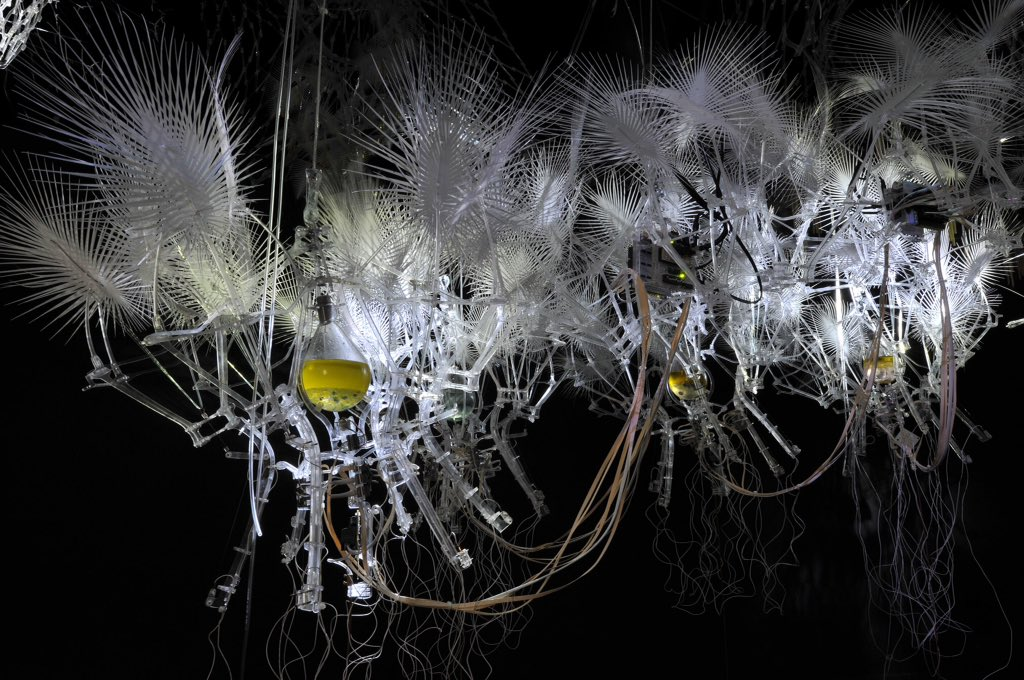
\includegraphics[width=\columnwidth]{images/sentient.jpeg}
\caption{Sentinent Architecture: Source: \url{https://nicolatriscott.files.wordpress.com/2016/03/caaqt-euyam-jpm.jpg}} 
\end{figure}

\section{Introduction}

What is it

\section{Existing Deployments}

list	existing deployments

\section{Impact}

why is it important

not only science, 

\section{Integration into Cloud Computing and Big Data}

how dos it for to cloud computing and big data (Gregor can do that)


\section{Development}
S Architecture in practice


\subsection{Snowwhite and the Seven$^{+1}$ Dwarfs}

The ISE department at Indiana University has obtained eight dendrites
that were assambled by a number of students so they can be used in
class and in research projects. These dendrites can be accessed in
Smith Research Center and allow students and faculty members to
experiment with them. They are bare dendrites and have no
electronics on them. Hence, you will need a hardware device to
interact with.

The reason we named them \textit{Snowwhite and the Seven$^{+1}$ Dwarfs}
is based on the fact that the dendrites are white, and they need to be
interact with  somone. Beacuse of the white color we name the controll
unit snowwhite. The dendrites that are interacting with it are called
dwarfs as this just fits to the name snowwhite. As we actually have 8
and not 7 we added $^{+1}$.


We do not recommend to directly attach the
wires to boards, as they will draw too much power and destroy the
boards. Instead you will need a relay that you controll that itself
controlls the dendrite These can be:

\begin{description}

\item[Arduino:] These boards very simple but provide relative good
  protection of the output links. The disadvantage is that its
  interface is in C.

\item[Teensy] Whatever is now on it TBD

\item[Raspberry Pi] We recommend to use a Raspberry Pi as it has a
  great operating system and is more suited for additional analysis of
  data within an Edge Computing network than the other two choices. It
  also allows you to use python which is clearly a pluss as most of
  the material presented here are in Python.

\end{description}


\begin{figure}
\centering
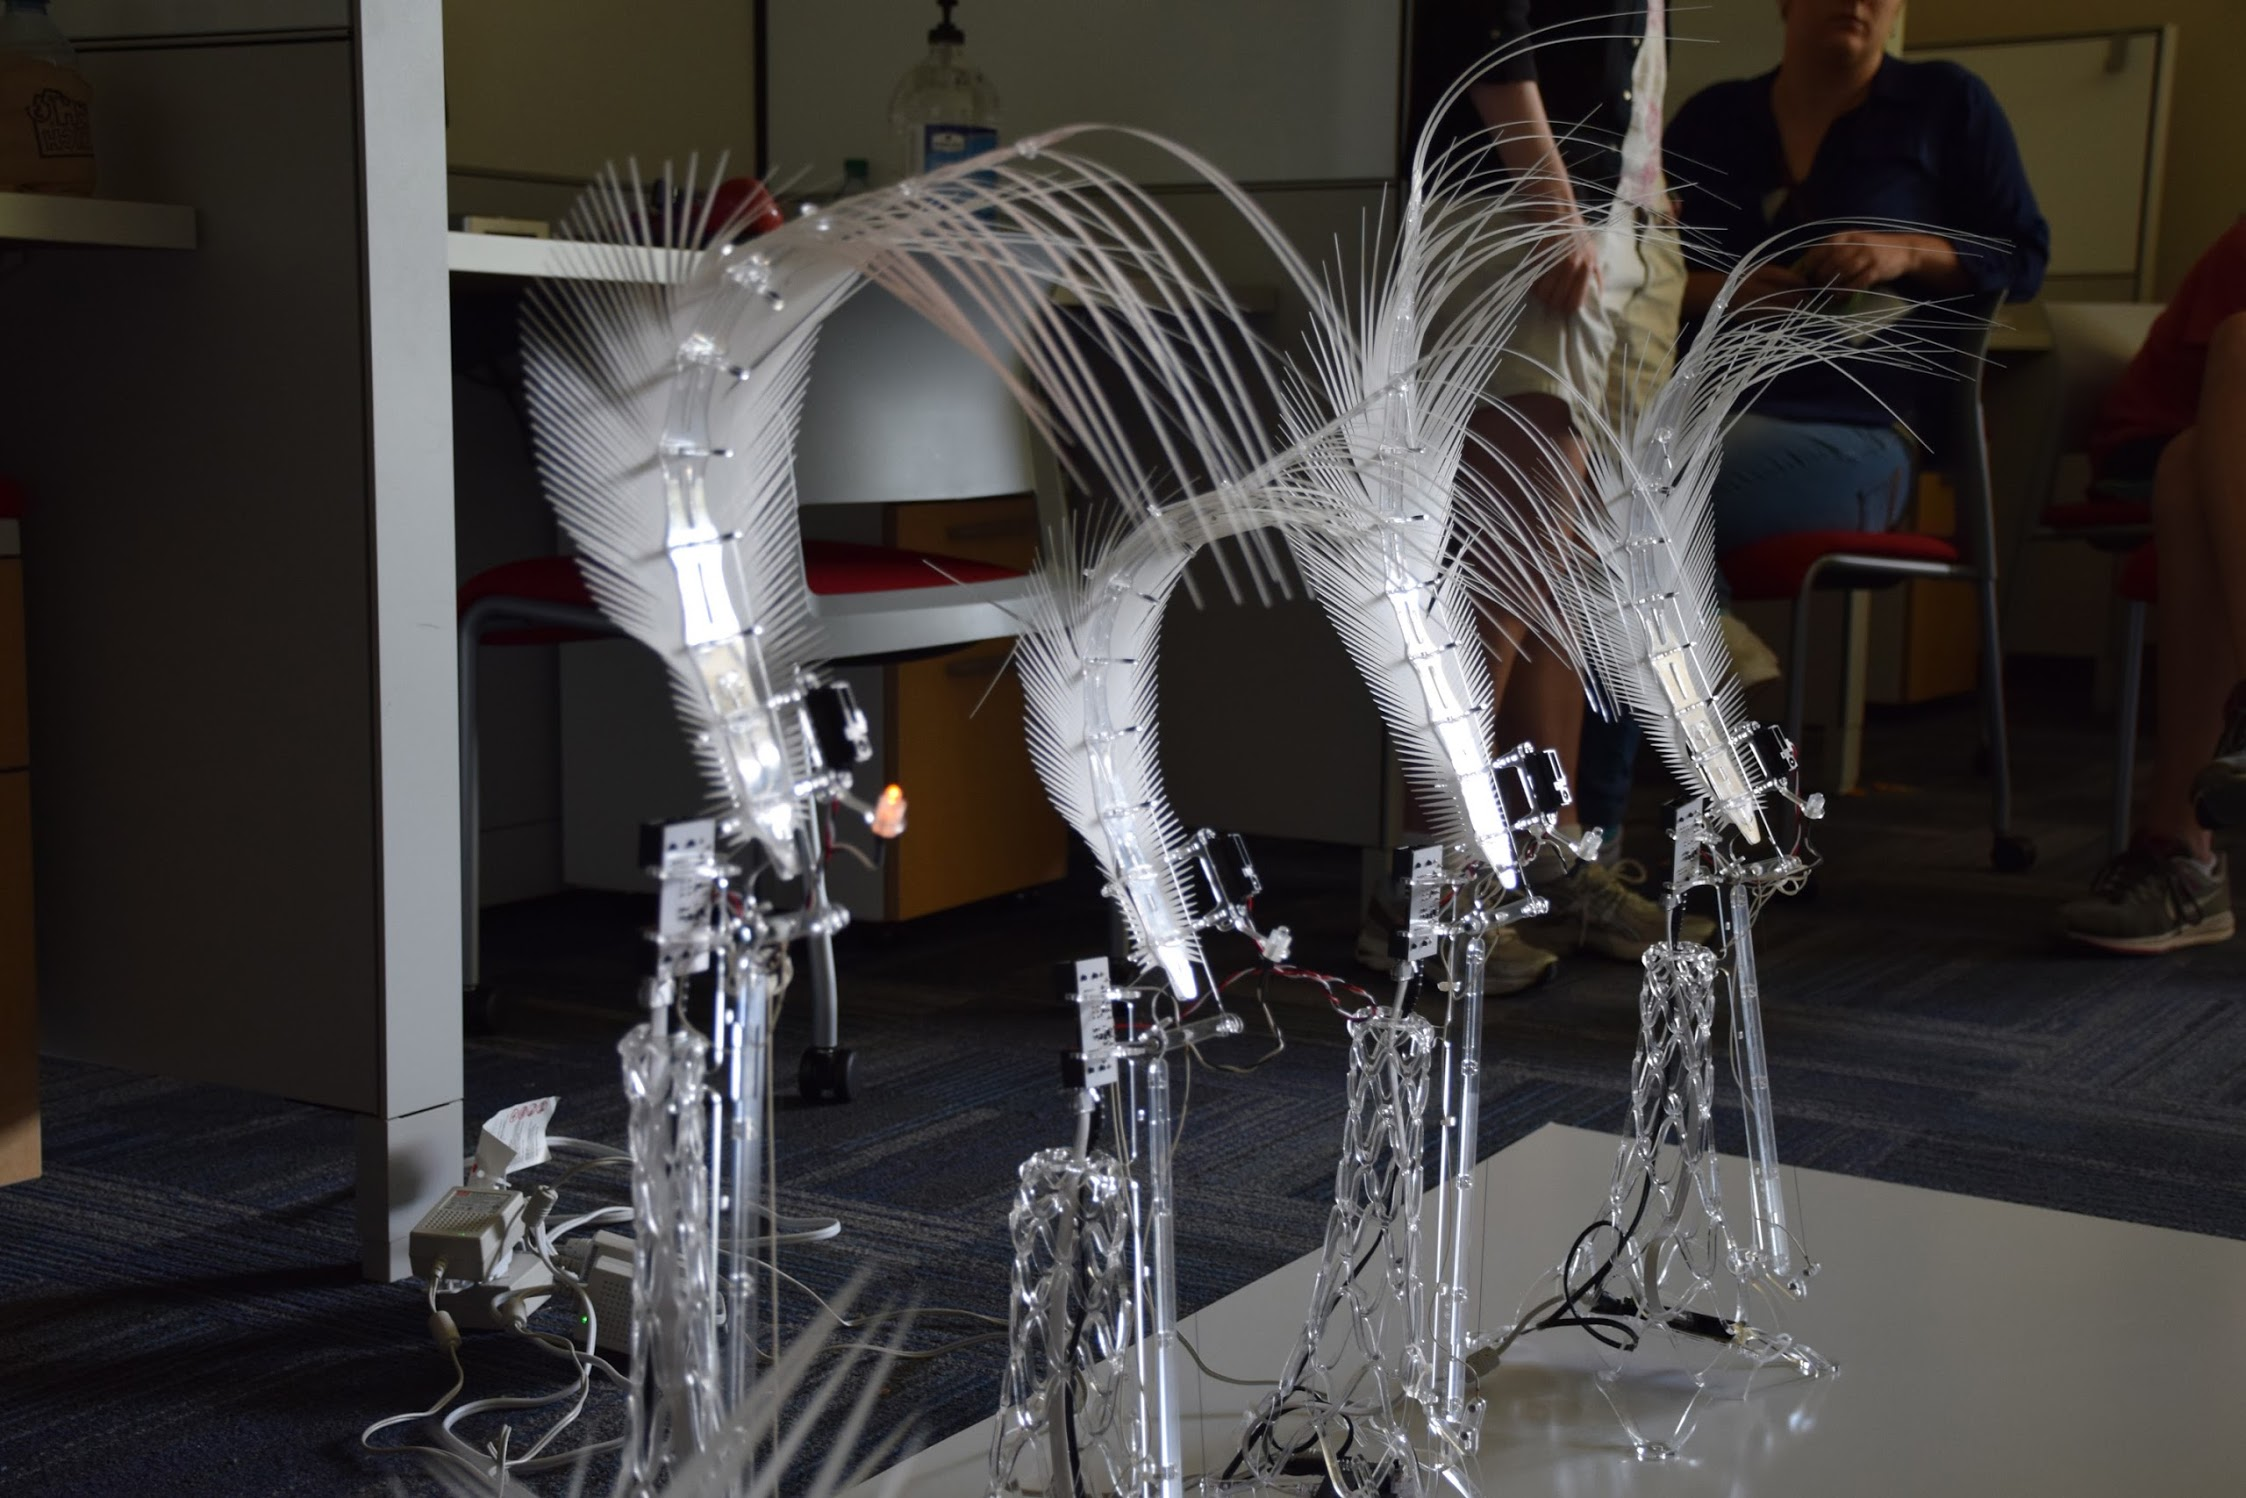
\includegraphics[width=\columnwidth]{images/snowwhite.jpg}
\caption{Snowwhite and the Seven$^{+1}$  Dwarfs}
\label{F:snowwhite}
\end{figure}


\subsection{Liddy Hall Installation}

architecture drawing


\section{Sentinent Cloudmesh}

	Gregor provides introduction to cloudmesh (probably just pointer to other section)

	Gregor provides introduction to cloudmesh.pi 

	Introduction to parallel programming in python (TBD)

	Towards the Cloudmesh Parallel S development environment


\paragraph{Snowwhite and the Seven$^{+1}$ Dwarfs}

Test environment (8 dendrites)

\paragraph{Liddy Hall}

Andreas dsecribes how we program them 

(Andreas provides)


than we use cloudmesh to interface with them, maybe we need to just
show how we integrate them into mqtt (this is snowhwite) and than we  
can progrem them from another pi

	Test environment Liddy hall 

\section{Alternative Boards}

\subsection{Mega 2560}

``The MEGA 2560 is designed for more complex projects. With 54 digital
I/O pins, 16 analog inputs and a larger space for your sketch it is
the recommended board for 3D printers and robotics projects. This
gives your projects plenty of room and opportunities.'' 
\url{https://store.arduino.cc/usa/arduino-mega-2560-rev3}
A nice case such as the one offered at Amazon will provide good
protection \url{https://www.amazon.com/Eleduino-Arduino-Mega-2560-Enclosure/dp/B016QE46RQ}


\begin{figure}
\centering
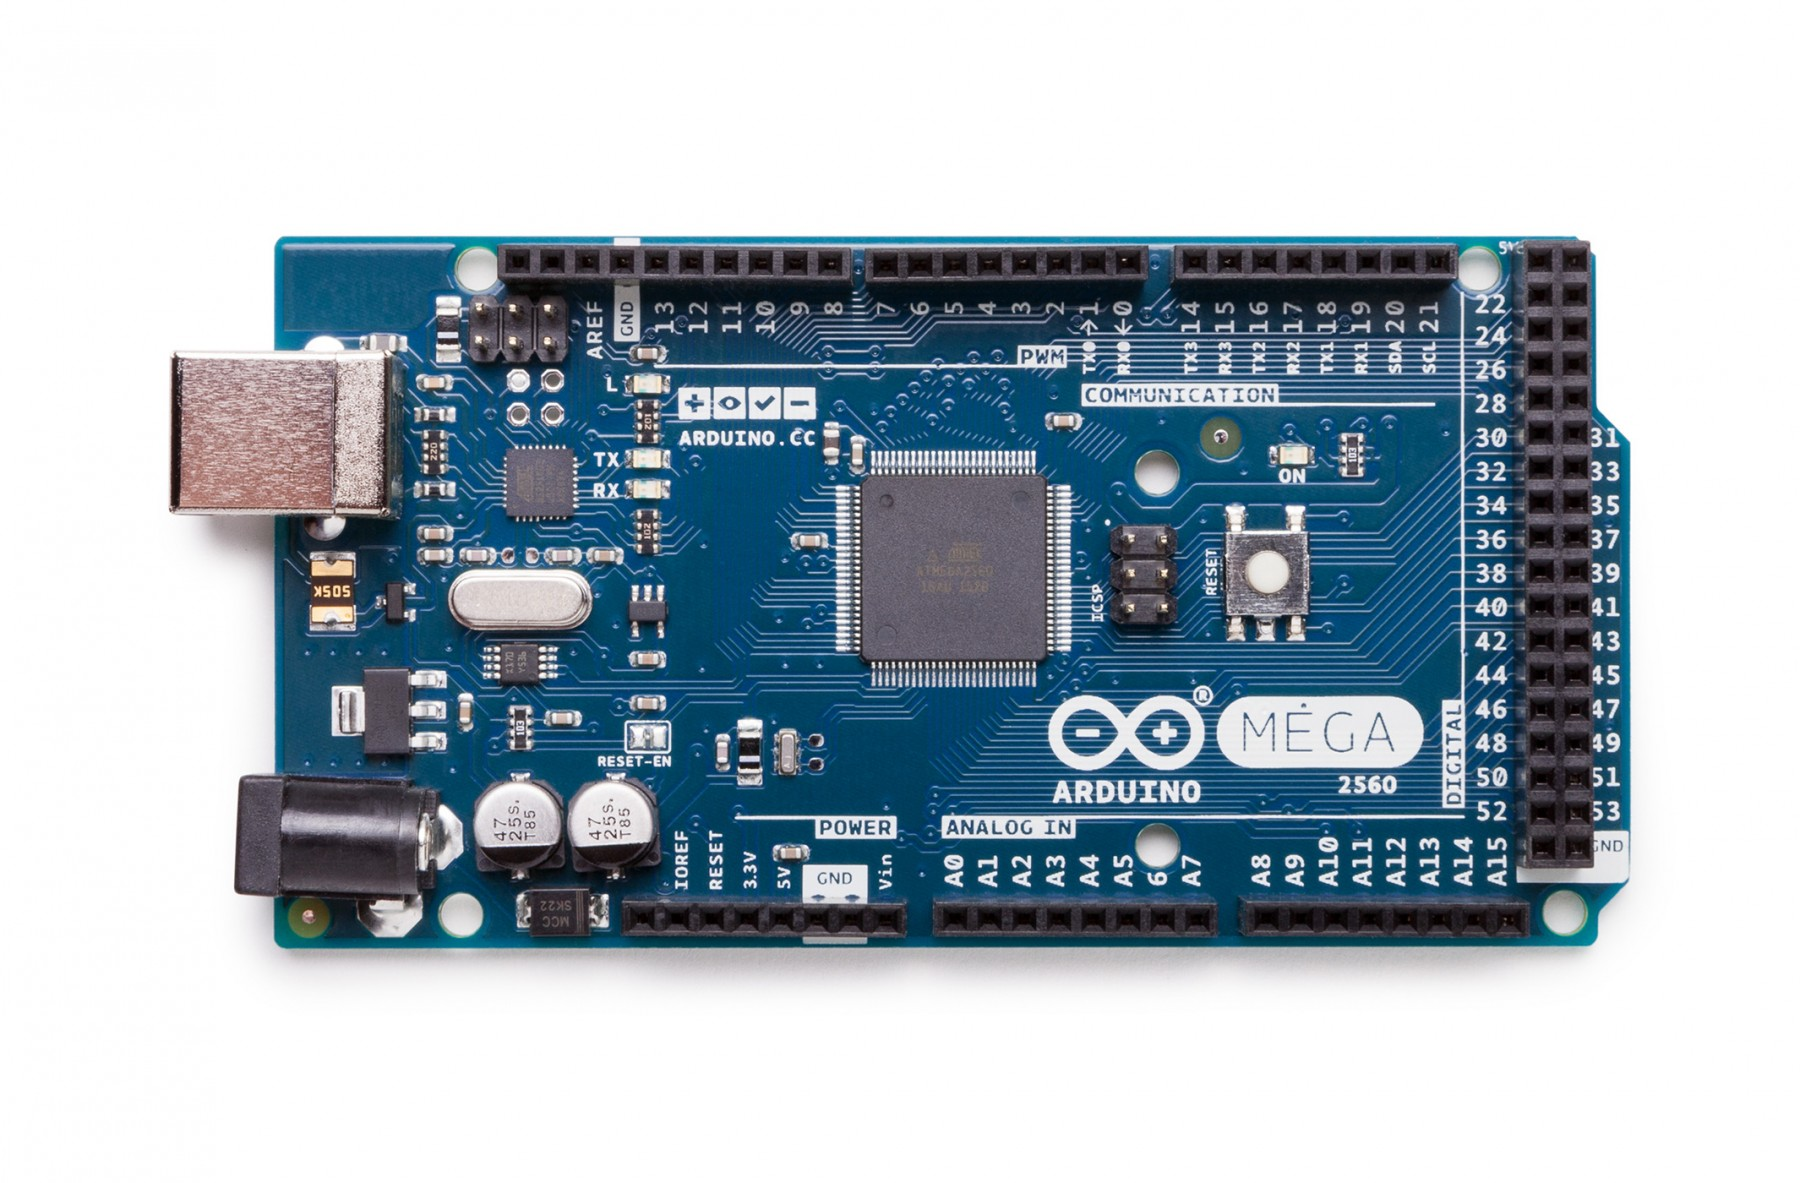
\includegraphics[width=0.25\columnwidth]{images/mega2560.jpg}
\caption{MEGA 2560}
\label{F:mega2560}
\end{figure}


\subsection{Programming with Teensy}

``The Teensy is a complete USB-based microcontroller development
system, in a very small footprint, capable of implementing many types
of projects. All programming is done via the USB port.'' Source: \url{https://www.pjrc.com/teensy/}

Current state of programming (whateverthey have)

Which version



\section{Exercises}

\begin{description}

\item[Sentinent.1] Build dendrite. In this excersise you will be
  building a dendrite that you can add to the available pool of dendrites.
\item[Sentinent.2.1] Develop cloudmesh sensor/actuary. In this excersise
  you will be developing an actuator ar sensor interface in object
  oriented programming methodology. You can see many examples in
  cloudmesh.py on github,com. You will pick a sensor you have access
  to and that is not already included in cloudmesh.pi. 
\item[Sentinent.2.2] If you do
  prefer using another board, the option may exist do develp an
  interface for the sensor or actuator for this device. If OO
  programming is not available for that board, a clean design based on
  functions must be provided. However we believe this is mor complex
  than using the Pi. 
\item[Sentinent.3.1] Develop an mqtt based event publisher and
  subscription service. Use first LEDs to test your service before you
  hook up relays and dendrites.
\item[Sentinent.3.2] Hook up the dendrites to mqtt and controll them
\item[Sentinent.4] Develop sensors that interact with the dendrites
\item[Sentient.5] Explore the Page at
  \url{https://www.intorobotics.com/alternative-arduino-boards/} that
  lists a number of PI/Arduino alteranative boards provide a non
  plagiarized table for this chapter and evaluate which could be
  viable alternatives. If you have one of them we like you to provide
  a documentation on how to integrate them with the dendrites.

\end{description}

 